% ICASSP-style course paper built from the local ICASSP 2026 template.
\documentclass{article}
\usepackage{spconf,amsmath,graphicx,booktabs,url}
\makeatletter
\setlength{\@fptop}{0pt}
\setlength{\@fpsep}{10pt}
\setlength{\@fpbot}{0pt plus 1fil}
\setlength{\@dblfptop}{0pt}
\setlength{\@dblfpsep}{10pt}
\setlength{\@dblfpbot}{0pt plus 1fil}
\makeatother
\renewcommand{\topfraction}{0.95}
\renewcommand{\bottomfraction}{0.95}
\renewcommand{\textfraction}{0.06}
\renewcommand{\floatpagefraction}{0.80}

\title{FROZEN PRETRAINED SPEECH REPRESENTATIONS IMPROVE LOW-RESOURCE ASR BUT REMAIN NOISE-SENSITIVE}

\name{Haowen Xu \qquad Yuchen Jiang \qquad Jiajun Wang}
\address{Shanghai Jiao Tong University\\
Student IDs: Haowen Xu 524031910714; Yuchen Jiang 524031910685; Jiajun Wang 524531910009}

\begin{document}
\ninept

\maketitle

\begin{abstract}
Low-resource automatic speech recognition (ASR) often has to generalize from clean supervision to noisy test audio. This paper introduces a controlled, CPU-friendly robustness protocol using 128 labeled LibriSpeech utterances for training and a clean/noisy evaluation set with 32 base utterances reused across SNR conditions. We compare a from-scratch log-mel BiLSTM-CTC model, a frozen wav2vec 2.0 base representation with a lightweight CTC head, a frozen ASR-fine-tuned wav2vec 2.0 encoder with the same head, and a pretrained wav2vec 2.0 CTC reference. The log-mel baseline saturates at 100\% WER, while the ASR-fine-tuned frozen representation reaches 5.5\% clean WER and 7.3\% WER at 20 dB. Its WER still rises to 44.1\% at 10 dB and 86.9\% at 5 dB. The protocol and edit-count analysis show that pretrained representations can rescue clean and mild-noise low-resource ASR, but severe additive noise remains a dominant failure mode.
\end{abstract}

\begin{keywords}
automatic speech recognition, low-resource ASR, noise robustness, wav2vec 2.0, CTC
\end{keywords}

\section{Introduction}
\label{sec:intro}

Automatic speech recognition (ASR) systems are often trained and evaluated under cleaner conditions than those faced in practical use. Background noise, channel variation, and scarce labeled speech can interact badly: a small supervised model may not learn a stable acoustic-to-character mapping, and additive noise can further perturb the cues it relies on. Low-resource noisy evaluation is therefore a useful stress test for the value and limits of pretrained speech representations.

Self-supervised and pretrained speech models such as wav2vec 2.0, HuBERT, and WavLM learn contextual frame representations from large speech corpora before downstream supervision \cite{baevski2020wav2vec2,hsu2021hubert,chen2022wavlm}. These representations are attractive when downstream labels are scarce, but full end-to-end fine-tuning is costly for a CPU-only course project. This motivates a narrower question: how much robustness can be obtained by freezing a pretrained encoder and training only a lightweight CTC head?

This paper answers that question with an independently designed stress-test protocol rather than a new ASR architecture. We train downstream models on 128 clean utterances and evaluate the same evaluation utterances under clean, 20 dB, 10 dB, and 5 dB additive-noise conditions. The design combines frozen continuous SSL representations, a matched lightweight CTC head, from-scratch and pretrained reference systems, and edit-type error decomposition. Across four systems, the result is clear: from-scratch low-resource ASR collapses, ASR-pretrained frozen representations recover clean and mild-noise recognition, and severe 5 dB noise remains a major failure case.

\section{Related Work}
\label{sec:related}

Connectionist temporal classification (CTC) provides a standard objective for sequence labeling when frame-level alignments are unavailable \cite{graves2006ctc}. In ASR, CTC trains acoustic models directly from utterance-level transcripts by marginalizing over monotonic alignments between acoustic frames and output tokens. We use CTC for all locally trained systems so that feature representations, rather than decoder differences, remain the main variable.

LibriSpeech is a widely used English read-speech benchmark derived from public-domain audiobooks \cite{panayotov2015librispeech}. Modern ASR systems usually train on hundreds or thousands of hours. This project intentionally restricts supervision to a much smaller subset, so the setup should be read as a low-resource stress test rather than a full-scale LibriSpeech benchmark.

Self-supervised speech pretraining has become a dominant approach for reducing labeled-data requirements. wav2vec 2.0 learns contextualized speech representations through a contrastive objective over masked latent speech units \cite{baevski2020wav2vec2}. HuBERT and WavLM extend this line of work with masked unit prediction and broader speech-processing objectives \cite{hsu2021hubert,chen2022wavlm}. Our experiments use Hugging Face Transformers implementations \cite{wolf2020transformers} of wav2vec 2.0 checkpoints and focus on frozen-feature use, which is cheaper than full fine-tuning and easier to reproduce on CPU.

\section{Experimental Setup}
\label{sec:setup}

\subsection{Data and Noise Protocol}
\label{ssec:data}

The experiments use a Mini LibriSpeech-style local subset generated from LibriSpeech manifests. The training set contains 128 clean train-clean-5 utterances, and the evaluation set contains 32 dev-clean-2 utterances. Each evaluation utterance is tested under four conditions: clean, 20 dB, 10 dB, and 5 dB. The final evaluation manifest contains 128 rows, with the same references reused across acoustic conditions.

Noisy evaluation waveforms are generated deterministically. For each clean waveform $x$ and synthetic noise vector $n$, the noisy signal is
\begin{equation}
    y = x + \alpha n,\qquad
    \alpha = \frac{\mathrm{rms}(x)}{\mathrm{rms}(n)10^{s/20}},
\end{equation}
where $s$ is the target SNR in dB. Training audio remains clean for all locally trained systems. This isolates the mismatch between clean low-resource supervision and noisy test-time conditions.

\subsection{Systems}
\label{ssec:systems}

Four systems isolate the effect of representation quality. First, the log-mel baseline extracts 80-dimensional log-mel features and trains a one-layer bidirectional LSTM CTC model from scratch. Second, the pure SSL ablation caches final-layer hidden states from wav2vec 2.0 base and trains the same lightweight BiLSTM-CTC head. Third, the ASR-pretrained encoder system caches final-layer hidden states from wav2vec 2.0 base-960h and trains the same CTC head. Fourth, a pretrained wav2vec 2.0 base-960h CTC model is evaluated directly as a reference.

The log-mel model is trained for 10 epochs with hidden dimension 256. The pure wav2vec 2.0 base hidden-state head is trained for 80 epochs with hidden dimension 128. The wav2vec 2.0 960h hidden-state head is trained for 30 epochs with hidden dimension 128. All local models use batch size 4, learning rate $10^{-3}$, character-level CTC targets, and greedy CTC decoding without a language model. Experiments run on CPU.

\subsection{Metrics}
\label{ssec:metrics}

The primary metric is word error rate (WER), computed as
\begin{equation}
    \mathrm{WER} = \frac{S + D + I}{N},
\end{equation}
where $S$, $D$, $I$, and $N$ are substitutions, deletions, insertions, and reference word count. Character error rate (CER) is computed analogously over characters. WER can exceed 100\% when insertions are large.

\section{Results}
\label{sec:results}

\begin{figure*}[t]
\centering
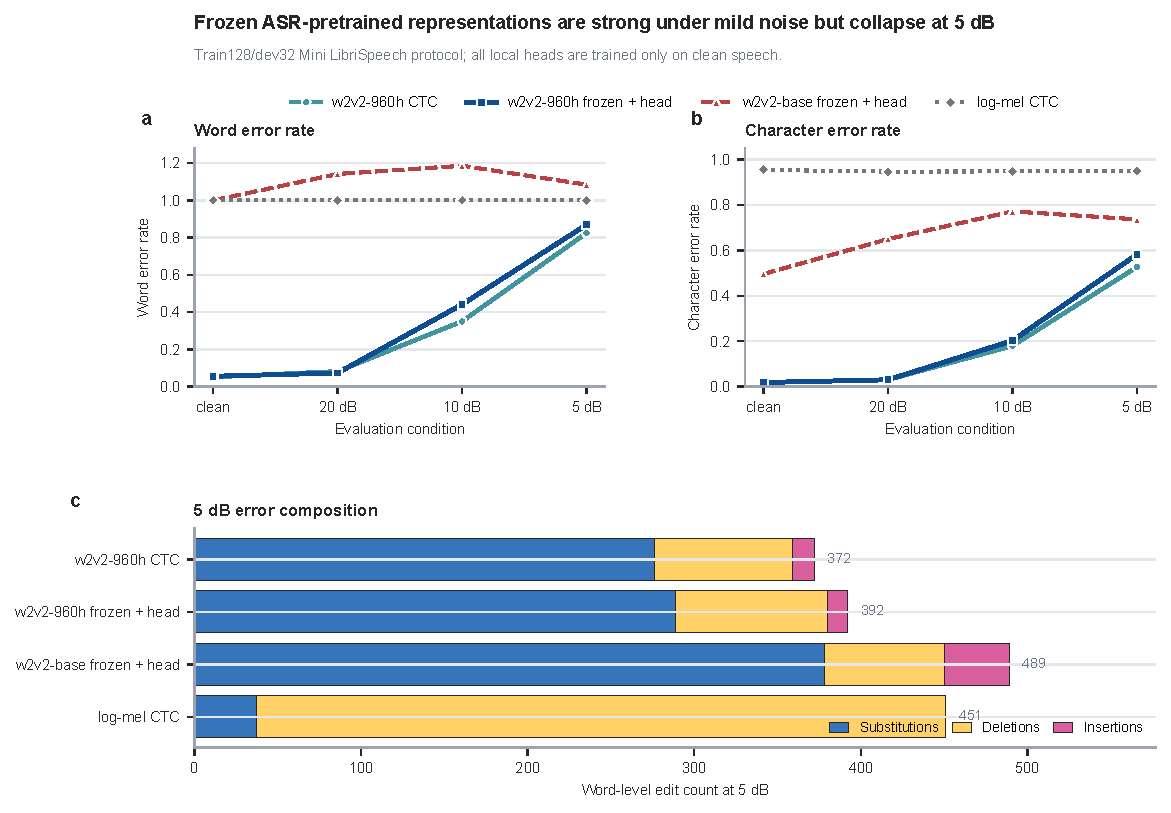
\includegraphics[width=0.98\textwidth]{figures/paper_robustness_main.pdf}
\caption{WER, CER, and 5 dB edit-count analysis. The ASR-pretrained frozen wav2vec 2.0 representation is strong on clean and 20 dB speech, but both pretrained systems degrade sharply as SNR drops to 10 dB and 5 dB. At 5 dB, substitutions dominate the errors of the stronger pretrained systems.}
\label{fig:robustness}
\end{figure*}

Table \ref{tab:wer_summary} summarizes WER across systems and SNR conditions. The from-scratch log-mel CTC model produces saturated WER in all conditions, indicating that the 128-utterance regime is too small for this model to learn a usable word-level recognizer. The pure wav2vec 2.0 base hidden-state model improves CER, but remains weak at the word level. In contrast, the wav2vec 2.0 960h hidden-state model reaches 5.5\% clean WER and 7.3\% WER at 20 dB, nearly matching the pretrained CTC reference in these easier conditions.

\begin{table}[t]
\centering
\caption{WER across clean and noisy evaluation conditions.}
\label{tab:wer_summary}
\footnotesize
\setlength{\tabcolsep}{2.5pt}
\begin{tabular}{lrrrr}
\toprule
System & Clean & 20 dB & 10 dB & 5 dB \\
\midrule
Log-mel CTC & 1.000 & 1.000 & 1.000 & 1.000 \\
w2v2-base + head & 1.000 & 1.142 & 1.187 & 1.084 \\
w2v2-960h + head & 0.055 & 0.073 & 0.441 & 0.869 \\
w2v2-960h CTC & 0.051 & 0.082 & 0.350 & 0.825 \\
\bottomrule
\end{tabular}
\end{table}

Figure \ref{fig:robustness} presents the same evidence as a robustness curve and error decomposition. The ASR-pretrained hidden-state head and the pretrained CTC reference are close under clean and 20 dB conditions. At 10 dB, WER rises to 44.1\% for the hidden-state head and 35.0\% for the pretrained CTC reference. At 5 dB, both systems fail on most words, reaching 86.9\% and 82.5\% WER, respectively. The frozen ASR-pretrained representation therefore transfers much of the clean-speech recognition ability, but does not by itself solve severe additive noise.

The CER results add a second boundary. The pure wav2vec 2.0 base hidden-state model has 49.6\% clean CER despite 100\% clean WER. This indicates partial character-level learning that does not become reliable word recognition. It also distinguishes the pure SSL ablation from the log-mel baseline, whose CER remains near 95\%. Pure SSL features are therefore not useless in this setting, but final-layer frozen features plus a small CTC head and 128 training utterances are insufficient.

\section{Discussion}
\label{sec:discussion}

The main result is a three-way distinction among feature regimes. The log-mel baseline shows that a small supervised CTC model can be too weak to serve as a meaningful robustness comparator when labeled data are extremely scarce. The pure wav2vec 2.0 base hidden-state model is better at the character level but still fails at word recognition. The ASR-fine-tuned wav2vec 2.0 960h encoder, even when frozen, provides a much more usable representation for a lightweight downstream head.

The severe-noise failure is not only a loss of confidence. Figure \ref{fig:robustness}(c) shows that, at 5 dB, the two strong systems are dominated by substitutions. The decoder emits plausible but wrong words rather than merely deleting uncertain speech. This is consistent with clean-trained acoustic representations being pushed across phonetic decision boundaries by strong additive noise. A practical robust ASR system therefore needs noise-aware training, augmentation, feature-layer selection, or full fine-tuning rather than frozen clean-speech representation reuse alone.

The independent design element is the combination of representation reuse and robustness diagnosis under strict compute constraints. Instead of only reporting a pretrained ASR score, the experiment asks whether a frozen SSL representation remains useful after low-resource clean supervision, where it fails as SNR decreases, and what type of edit errors drive that failure. This satisfies the course project's emphasis on self-supervised speech representations while keeping the method reproducible on CPU.

This interpretation has clear boundaries. The evaluation set contains only 32 base utterances, so the numbers should be read as a controlled pilot rather than a statistically definitive benchmark. The noise is deterministic synthetic noise instead of real environmental recordings. The pure SSL ablation uses only the final hidden layer, although intermediate layers may be better for phonetic transfer. Finally, the local CTC heads use greedy decoding without a language model, which simplifies comparison but may understate what a tuned ASR system could achieve.

\section{Conclusion}
\label{sec:conclusion}

This paper presented a CPU-friendly study of low-resource ASR robustness under controlled additive noise. With only 128 clean training utterances, a log-mel BiLSTM-CTC baseline collapses, and a pure wav2vec 2.0 base hidden-state head remains weak at the word level. Frozen hidden states from an ASR-fine-tuned wav2vec 2.0 960h model, however, produce strong clean and mild-noise results and nearly match a pretrained CTC reference. Severe 10 dB and 5 dB noise still causes large WER increases. The next step is therefore not simply to reuse frozen representations, but to combine them with noise-aware adaptation and evaluate on larger real-noise test sets.

\section{Reproducibility}
\label{sec:repro}

All experiments are implemented as local scripts with fixed manifests, cached feature files, and exported CSV metrics. The final configuration, result tables, and regenerated paper figures are stored with the project artifacts. The pure wav2vec 2.0 base download used \texttt{HF\_HUB\_DISABLE\_XET=1} when the Hugging Face xet download path stalled.

\clearpage
\raggedbottom
\bibliographystyle{IEEEbib}
\bibliography{references}

\end{document}
